\section{Experimental Work}
The following sections detail the research that TESLA has done in the field of TR WPT. These experiments are meant to accomplish several goals:

\begin{itemize}
    \item Characterize the behaviors of TR relevant to WPT applications
    \item Understand fundamental limitations of TR applied to WPT
    \item Create a baseline for which future work can be done
\end{itemize}

The general methodology for the experiments is described. Then, the purpose, methodology, and results of individual experiments are discussed individually.

\chapter{Methodology for Conducting Linear Time Reversal Measurements}
\label{ch:linear-meth}

The majority of our experiments take place within an enclosed, reflective cavity called the Gigabox: an aluminum box with a metallic foil scattering paddle to make the ray trajectories more ergodic. Ray chaos ensures that a propagating pulse will eventually reach every point in the environment, which insures that many transmission channels are simultaneously excited. This improves reconstruction fidelity. Up to five monopole antennas inject and extract electromagnetic signals from different ports in the enclosure depending on the experiment.

Our Time Reversal scheme consists of three pieces of microwave processing equipment and a desktop workstation. Interrogation pulses and time-reversed sona signals are created and broadcast using a Tektronix \texttt{AWG7052} arbitrary waveform generator feeding an Agilent \texttt{E8267D} Vector PSG microwave source. A digital storage oscilloscope (DSO, Agilent \texttt{DSO91304A}) is used to record waveforms of interest. MATLAB is used for signal processing and instrument control and coordination.

In many experiments, it is necessary to be able to ``read'' and ``write'' signals from the same port. Manually switching coaxial cables from the PSG to the DSO is slow and can destroy reconstructions, so we use four HP 8762C coaxial switches to reroute signals as required.

This hardware is laid out in Figure~\ref{fig:linear-gigabox}.

\begin{figure}[h!]
\centering
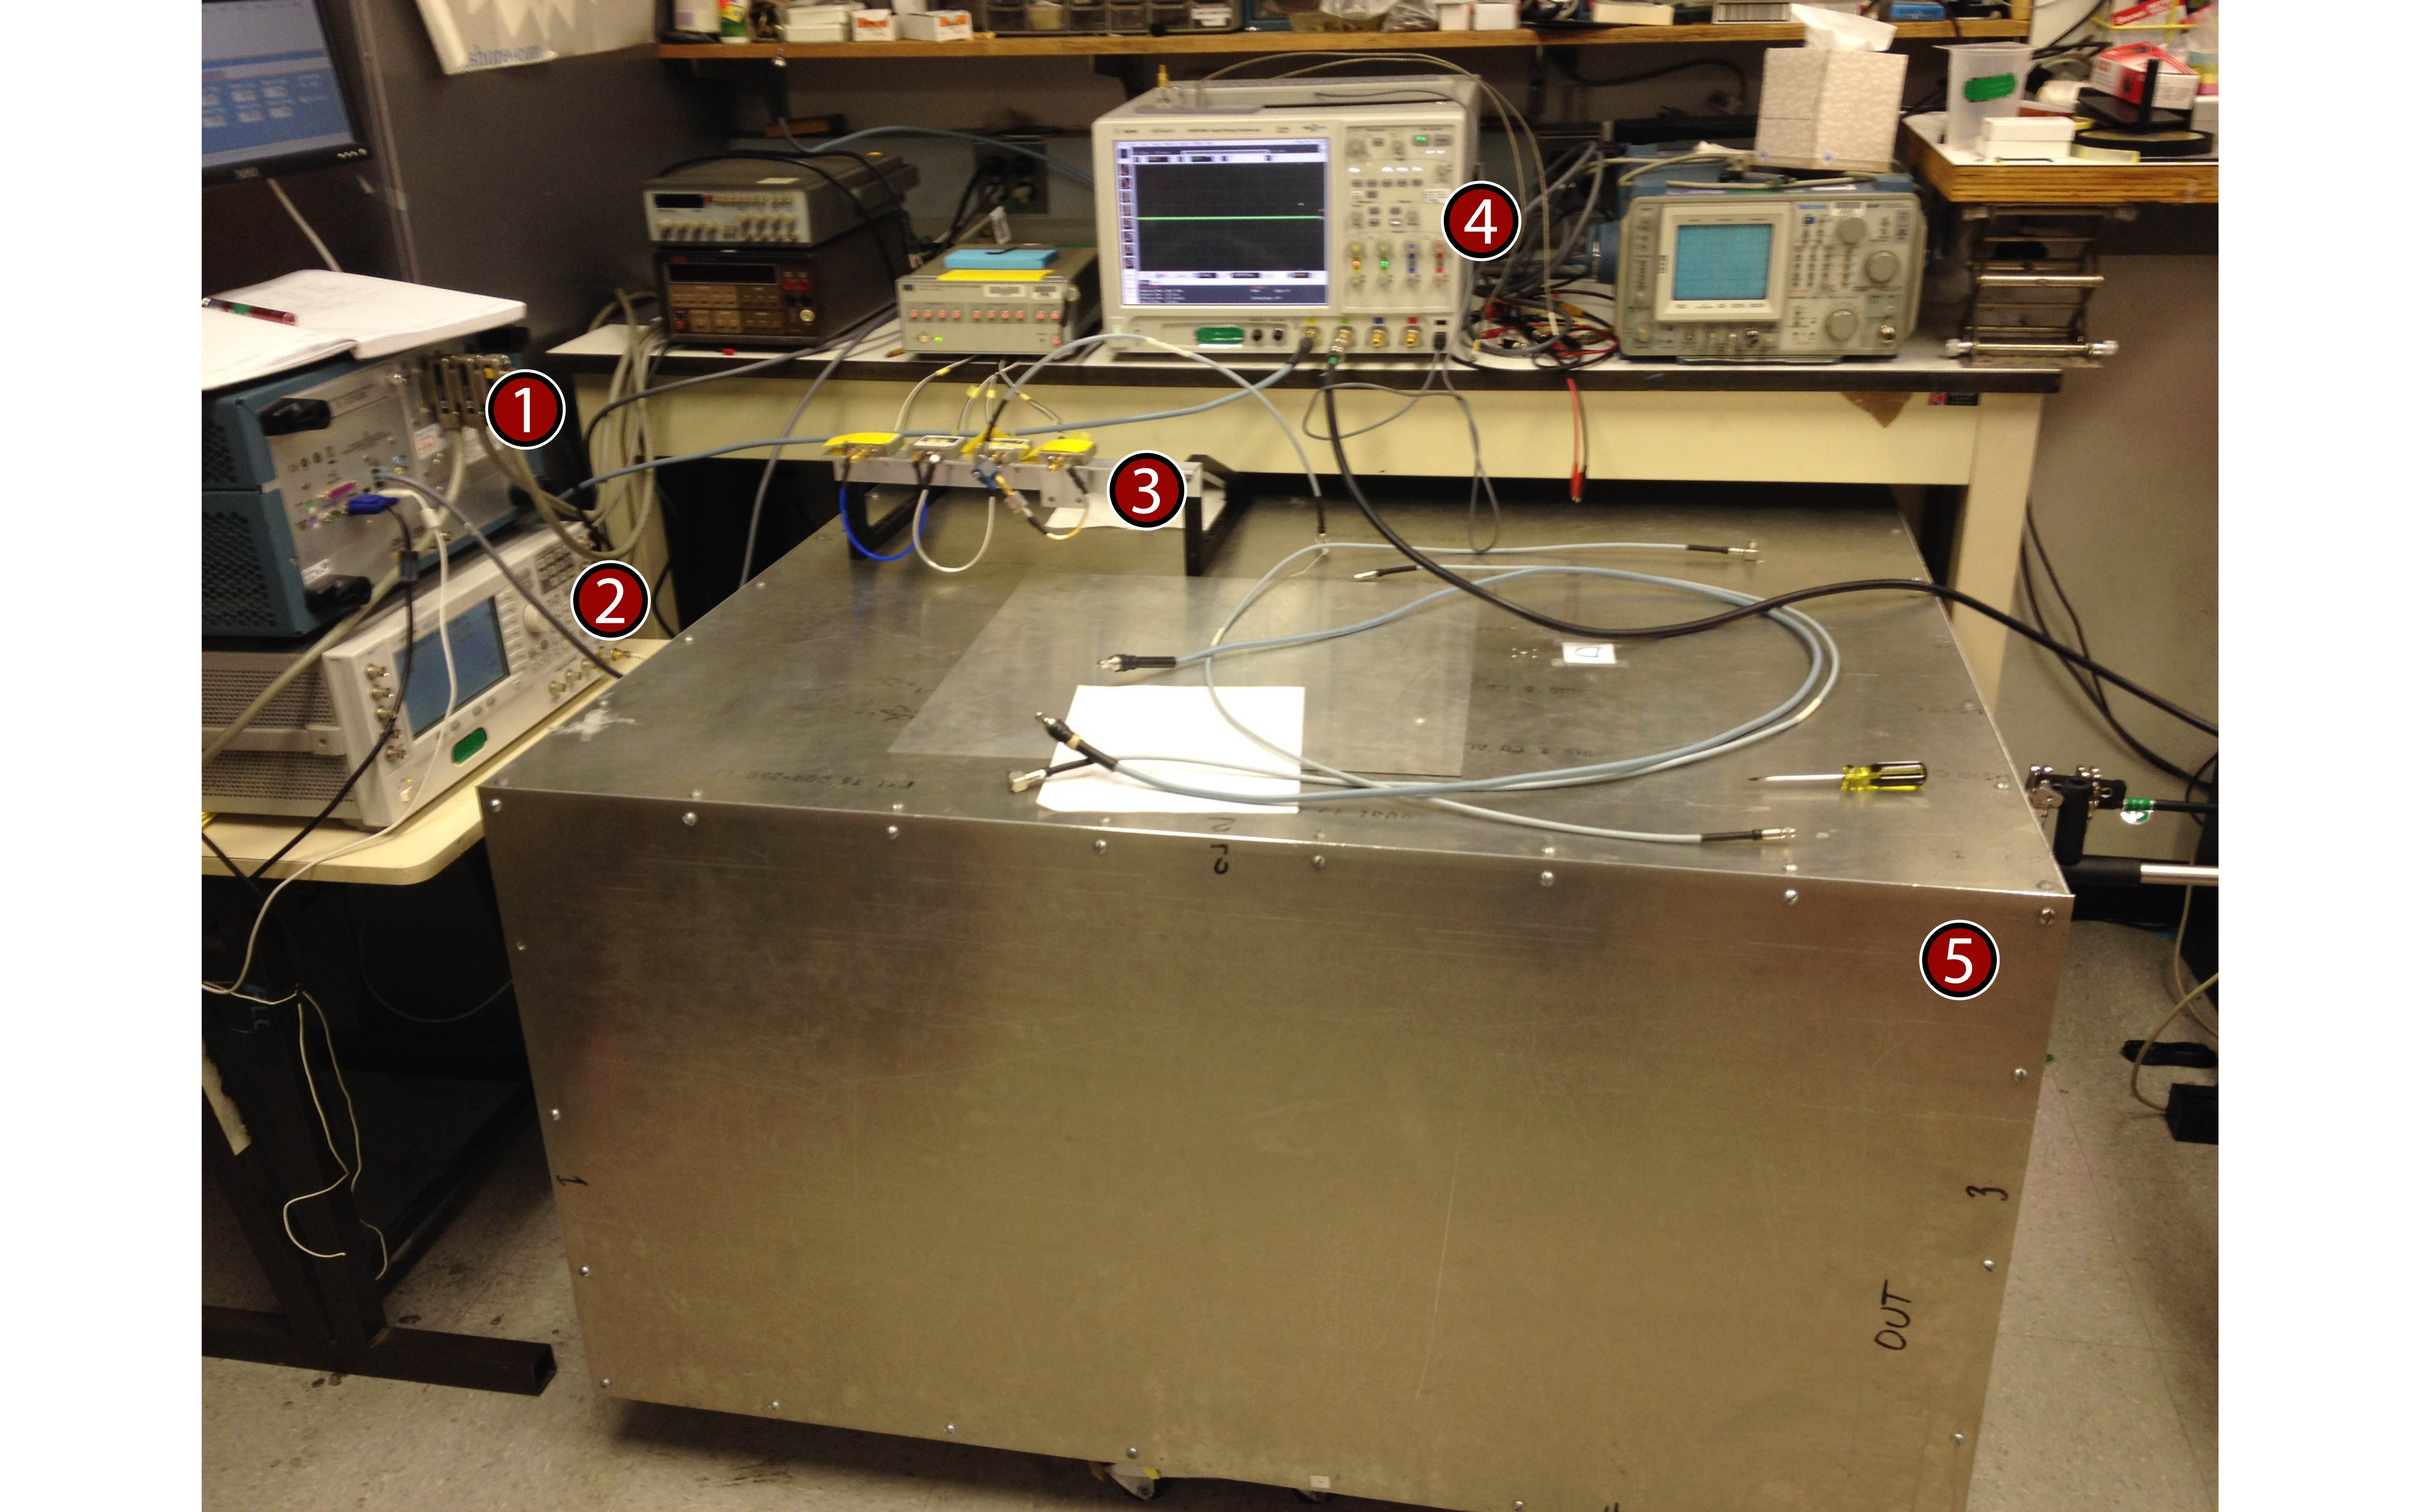
\includegraphics[width=0.85\textwidth]{linear/gigabox}
    \caption[Lab equipment setup]{Lab equipment setup: 1) Tektronix \texttt{AWG7052} Arbitrary Waveform Generator, 2) Agilent \texttt{E8267D} Vector PSG Microwave Source, 3) Array of four Hewlett-Packard 8762C coaxial switches, 4) Agilent \texttt{DSO91304A} Digital Storage Oscilloscope, 5) 1.06~$m^3$ aluminum ``Gigabox'' with interior conductive scattering paddle.}
    \label{fig:linear-gigabox}
\end{figure}

Our TR experiments fall into two main categories, linear and nonlinear. Linear TR (LTR) refers to any experiment that uses a single frequency. Nonlinear TR (NLTR) makes use of harmonic reflections from the target to provide a means for isolation and targeting, a process similar to how we would envision a TR based WPT system to work.  It is experimentally much simpler to create reconstructions with LTR than with NLTR, so we use it for experiments investigating the behavior of the waves rather than the behavior of the target.

This section concerns LTR experiments. Conceptually, our general process for LTR in the Gigabox is as follows: we broadcast a Gaussian interrogation pulse from one port, serving as a transmitter. This interrogation pulse reverberates and echoes around the reflective cavity. Another port, designated as the receiver, records the multipath sum of these reverberations with the oscilloscope. This summed signal is named a sona, and inherently contains information relating to the size and shape of the interrogation pulse, the location of any scattering media in the environment, and the location of both ports. That sona is reversed in the time domain and subsequently rebroadcast from the transmitting port. The signal will travel through the same multipath channels and reconstruct a time reversed version of the original interrogation pulse upon the receiver, with some additional noise. This process is illustrated in Figure~\ref{fig:linear-ltr}.

\begin{figure}[h!]
\centering
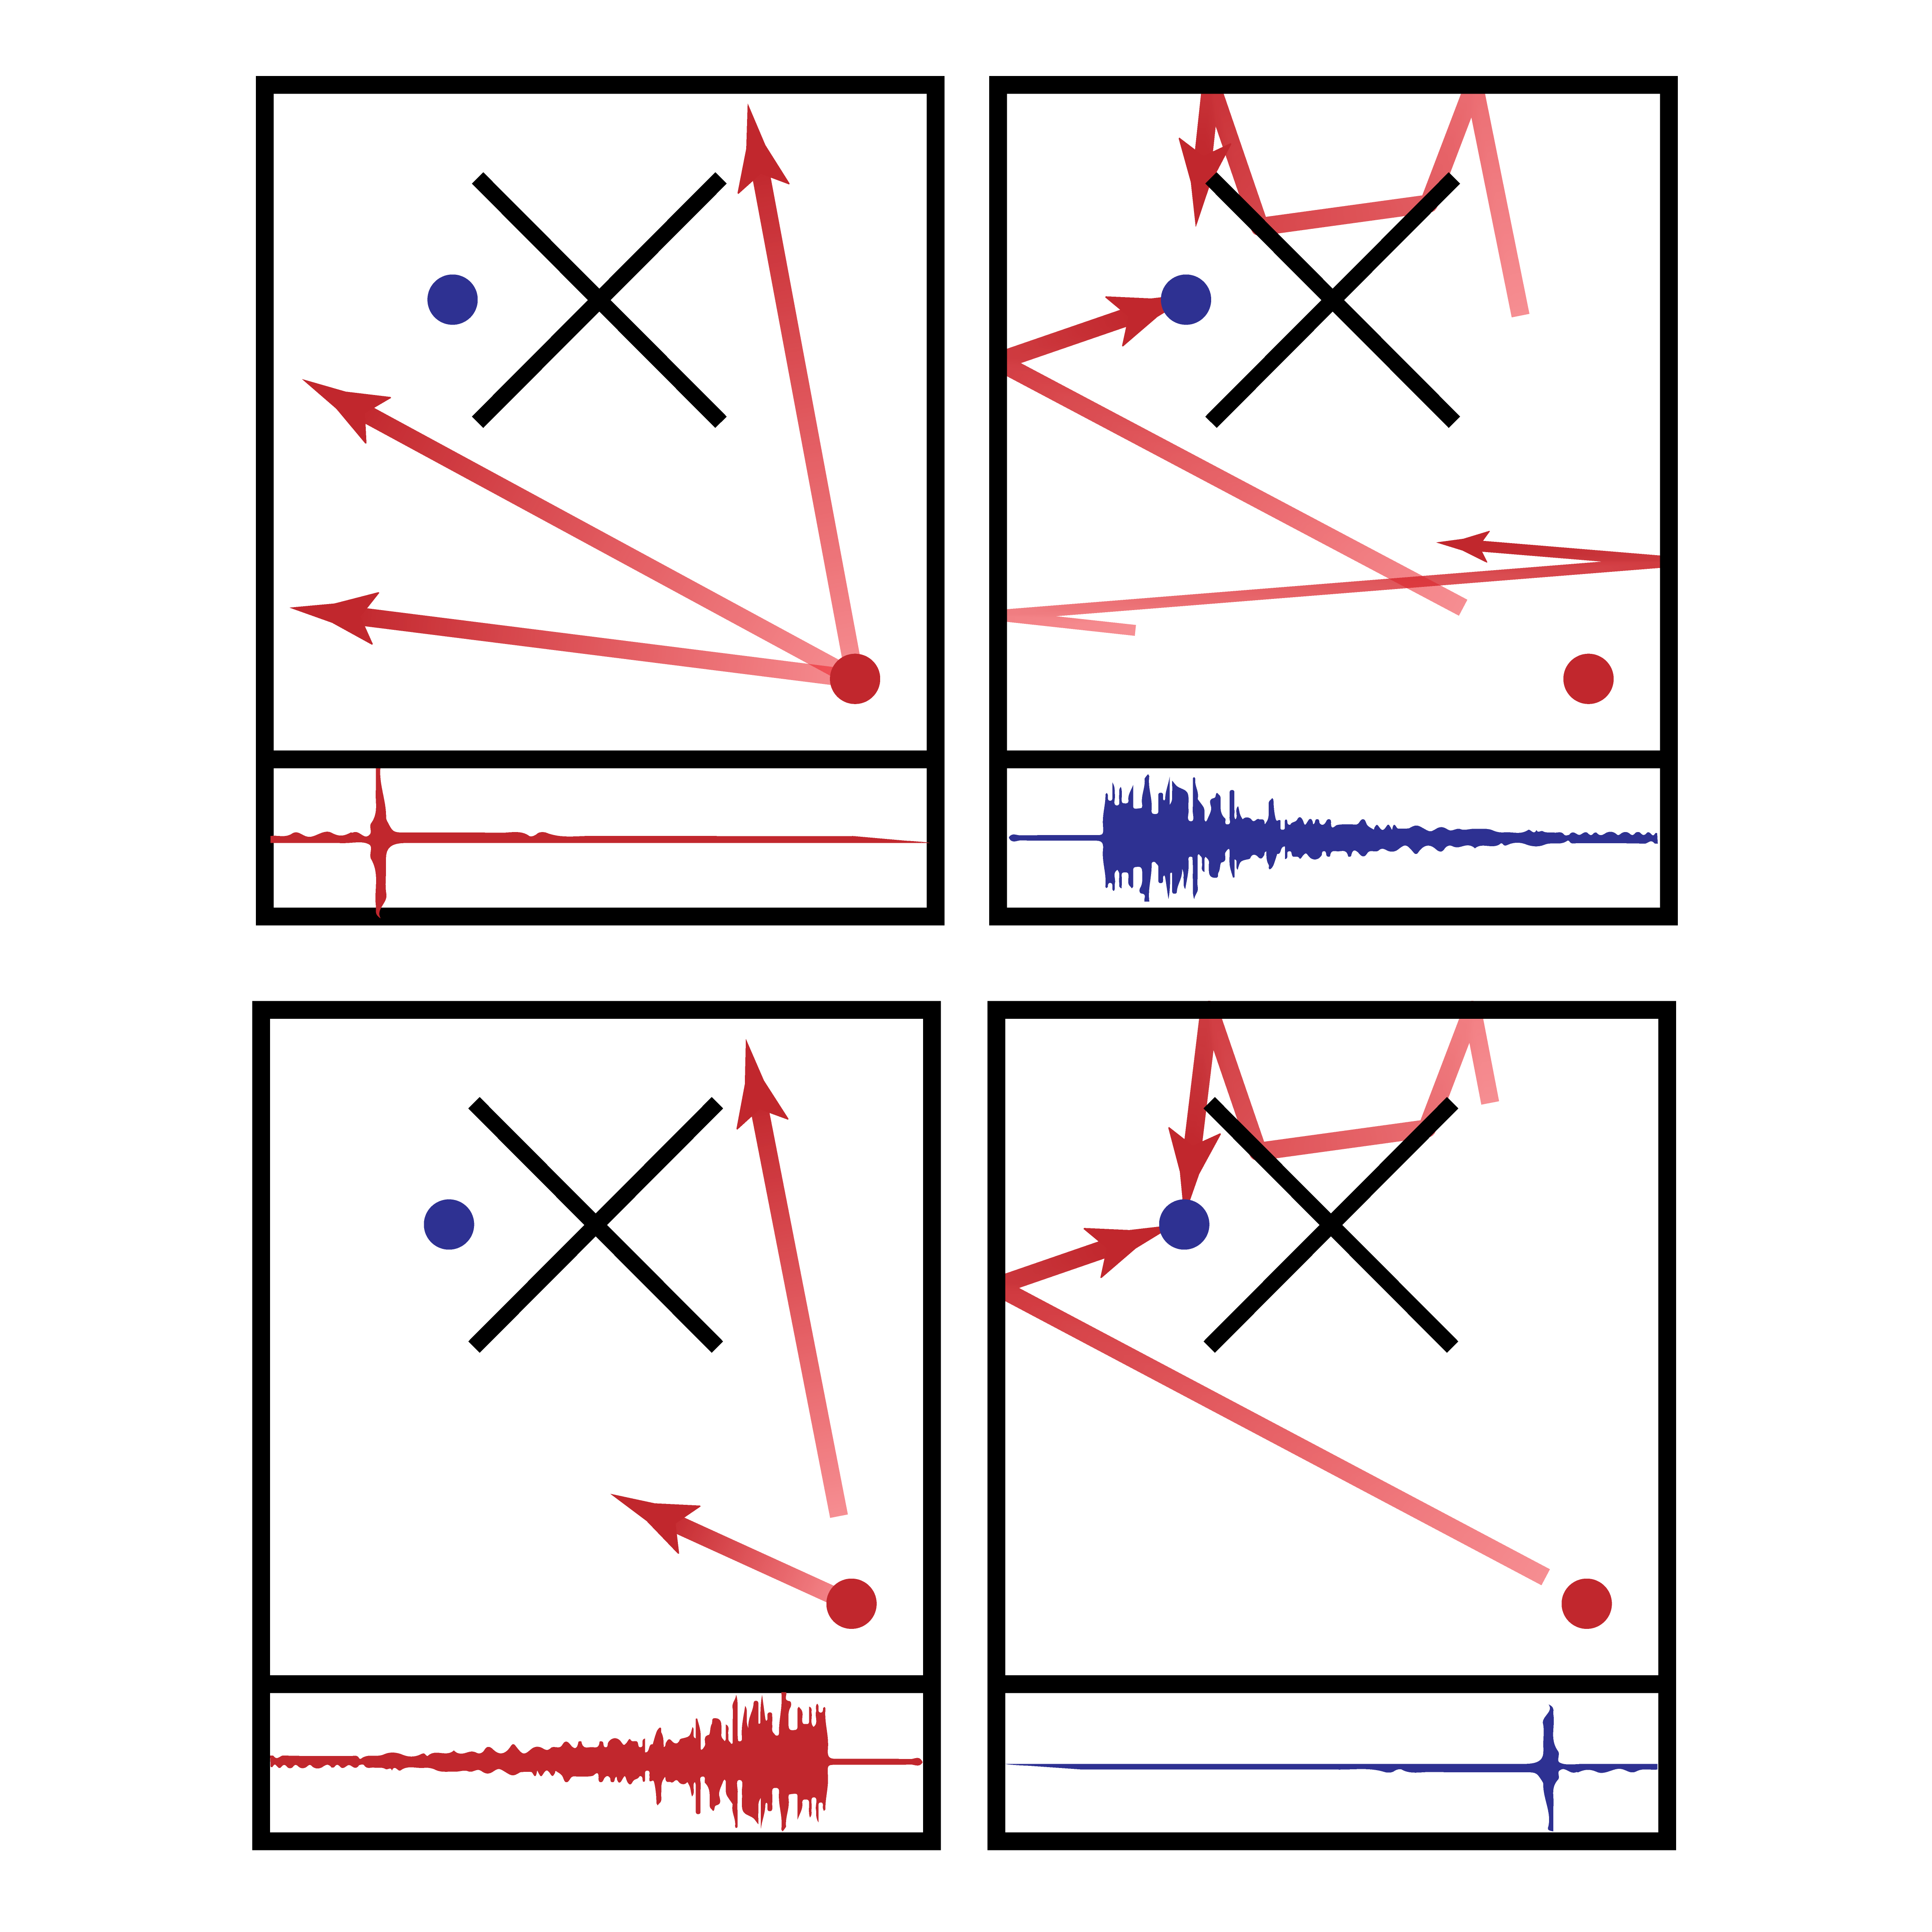
\includegraphics[width=0.85\textwidth]{linear/ltr}
    \caption[Conceptual overview of linear time reversal]{Reading order from top left: Visualization of the linear time reversal process.}
    \label{fig:linear-ltr}
\end{figure}

Since this LTR process is well-suited to creating reconstructions of Gaussian waveforms, we used it for three experiments to examine characteristics and modifications of LTR itself. These were: 
\begin{itemize}
    \item Overlaying sonas to create more closely spaced reconstructions
    \item Mapping the spatial profile of a reconstruction
    \item Repeatedly retargeting the reconstructions upon a moving antenna
\end{itemize}
The experiments, results, and discussions for these sections are presented respectively as "Overlapping Reconstructions", "Spatial Profiling", and "Moving Reconstructions" below. The experience the team gained by performing these experiments and formulating results was invaluable in constructing and performing our later work with Nonlinear Time Reversal (NLTR). They also demonstrate important ideas regarding the transmission of large amounts of power to the receiver.
